\chapter[Metodología]{
  \label{chp:metodologia}
  METODOLOGÍA
}
\thispagestyle{numberingStyle}
\pagestyle{numberingStyle}


Para el desarrollo de este proyecto se ha escogido una metodología basada en el Proceso Unificado. Esta metodología nos permite obtener un producto de alta calidad gracias a su carácter iterativo e incremental. De manera que, en cada ciclo o iteración, el producto es revisado y mejorado.


\section{Características}
El Proceso Unificado es un marco de desarrollo software caracterizado por estar dirigido por casos de uso, centrado en la arquitectura y por ser iterativo e incremental.

\subsection{Dirigido por casos de uso}
Un caso de uso es un fragmento de funcionalidad del sistema que proporciona un resultado de valor a un usuario. Los casos de uso modelan los requerimientos funcionales del sistema y todos juntos constituyen el  modelo de casos de uso.

Los casos de uso también guían el proceso de desarrollo (diseño, implementación y prueba). Basándose en los casos de uso, los desarrolladores crean una serie de modelos de diseño e implementación que llevan a cabo. De este modo, los casos de uso no son solo una herramienta para especificar los requerimientos e iniciar el proceso de desarrollo, sino que también dirigen su diseño, implementación, pruebas, etc...

\subsection{Centrado en la arquitectura}
La arquitectura de un sistema software se describe mediante diferentes vistas del sistema en construcción. Se define arquitectura como el conjunto de decisiones significativas acerca de la organización de un sistema software, la selección de los elementos estructurales a partir de los cuales se compone el sistema y su composición.

Los casos de uso y la arquitectura están profundamente relacionados. Los casos de uso deben encajar en la arquitectura, y esta a su vez, debe permitir el desarrollo de todos los casos de uso requeridos, actualmente y a futuro.

De tal forma que, el arquitecto software desarrolla la forma o arquitectura a partir de la comprensión de un conjunto reducido de casos de uso fundamentales o críticos.

\subsection{Iterativo e incremental}
Se divide el desarrollo de un proyecto software en partes más pequeñas o mini proyectos. Cada mini proyecto es una iteración que supone un incremento. Las iteraciones hacen referencia a pasos en el flujo de trabajo, y los incrementos, a crecimientos en el producto.

Las iteraciones deben estar controladas de manera que se deben seleccionar y ejecutar de forma planificada. 

En cada iteración los desarrolladores identifican y especifican los casos de uso relevantes y crean un diseño utilizando la arquitectura seleccionada para implementar dichos casos de uso. Si la iteración cumple sus objetivos, se continúa con la próxima, si no, deben revisarse las decisiones previas y probar un nuevo enfoque.

\section{Ciclo de vida}
El Proceso Unificado se repite a lo largo de una serie de ciclos que constituyen la vida de un sistema.


\begin{figure}[H]

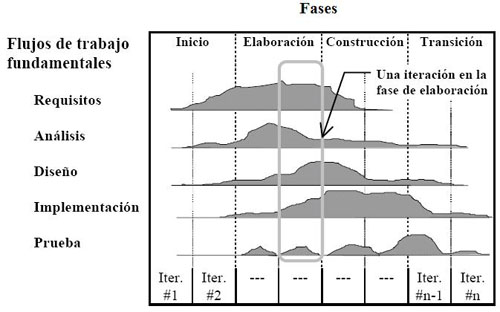
\includegraphics[
   keepaspectratio=true
]{./03_Met_Plan/01_Metodologia/diagramaProcesoUnificado.JPG}
\caption{Ciclo de vida - Proceso Unificado de Desarrollo}
\end{figure}


Cada ciclo consta de cuatro fases: \textbf{Inicio}, \textbf{Elaboración}, \textbf{Construcción} y \textbf{Transición}. Cada fase se divide en iteraciones, en las cuales se desarrolla, secuencialemte, una serie de disciplinas o flujos de trabajo como son, por ejemplo: \textit{Análisis, Diseño, Implementación y Pruebas.}

En la figura podemos observar que el ciclo de vida del Proceso Unificado presenta dos dimensiones:
\begin{itemize}
	\item Un eje horizontal que representa el aspecto dinámico del proceso conforme se va desarrollando. Expresado en términos de \textit{Fases, Iteraciones e Hitos}.
	\item Un eje vertical que representa el aspecto estático del proceso mediante las disciplinas o flujos de trabajo.
\end{itemize}


\subsection{Fase de inicio}
Durante la fase de inicio se desarrolla una descripción del producto final y se presenta el análisis de negocio.

El objetivo de esta fase es ayudar al equipo a decidir cuales son los verdaderos objetivos del proyecto.

\subsection{Fase de elaboración}
En esta fase se especifican la mayoría de los casos de uso del producto y se diseña la arquitectura del mismo. Se establece una firme comprensión del problema a solucionar.


\subsection{Fase de construcción}
Durante la fase de construcción se elabora el producto, de tal manera que la línea base de la arquitectura avanza hasta convertirse en el sistema completo. Al final de esta fase se obtienen todos los casos de uso implementados aunque pueden incluir defectos.


\subsection{Fase de transición}
La fase de transición hace referencia al período donde el software ya debe estar listo para ser instalado, probado y utilizado. Las iteraciones en esta fase continúan agregando características al software.


\section{Iteraciones}
\subsection{Iteración 1: Análisis de requisitos y diseño}

En esta primera iteración se determinará la planificación del proyecto, se realizará la recogida de requesitos y el modelado de casos de uso. También se especificará el diseño del sistema y se elaborará el diagrama de clases de la aplicación.


\subsection{Iteración 2: Base inicial del proyecto}
La segunda iteración implicará el comienzo del desarrollo del proyecto. Se preparán los entornos necesarios, se realizará una pequeña formación en las tecnologías que se emplearán y se preparará y configurará la base datos. Al hacer uso de APIs externas, en esta iteración, se configurarán para su posterior uso.


\subsection{Iteración 3: Usuarios}
La iteración 3, tiene como objetivo la implementación de las funcionalidades relacionadas con los usuarios de la aplicación. Se realizará el análisis y diseño, así como la implementación de la persistencia y lógica de negocio para la gestión de los usuarios. Finalmente, se realizarán las pruebas necesarias.


\subsection{Iteración 4: Rutas}
En esta iteración se realizará el análisis y diseño, la implementación de la persistencia y la lógica de negocio, y las pruebas necesarias para la gestión de las rutas en la aplicación.


\subsection{Iteración 5: Eventos}
Análogamente, en la iteración número 5, se realizará el mismo ciclo de acciones. Análisis y diseño, implementación de la persistencia y lógica de negocio, y pruebas, esta vez, para la gestión de eventos.



\subsection{Iteración 6: Servicios externos}
En esta iteración se llevará a cabo la gestión de las funcionalidades y datos obtenidos de las fuentes externas. Se realizará el análisis y diseño para la implementación de los servicios externos necesarios, se realizarán las modificaciones necesarias para el correcto funcionamiento de la librería Java de Foursquare, así como la implementación y pruebas necesarias para dichos servicios.


\subsection{Iteración 7: Lugares y categorías}
Se realizará análisis, diseño, implementación y pruebas para la gestión de lugares y categorías, cuyos datos serán obtenidos por los servicios definidos e implementados en la iteración anterior.


\subsection{Iteración 8: Capa servicios}
Para la iteración 8 se llevará a cabo el desarrollo de la capa de servicios del modelo. Se realizará el análisis, diseño, implementación y pruebas.


\subsection{Iteración 9: Autenticación y autorización}
En este iteración se llevará a cabo el proceso de autenticación y autorización de los usuarios. Se realizará el análisis y diseño, así como la implementación y pruebas necesarias.


\subsection{Iteración 10: Cliente móvil}
De igual forma, en esta iteración, se realizará anáisis, diseño, implementación y pruebas para la elaboración del cliente móvil. Se realizará también una formación en las tecnologías utilizadas en su creación, la implementación de las pantallas y controladores, y de los módulos de acceso de a los servicios previamente implementados.


\subsection{Iteración 11: Cliente web}
Iteración cuyo objetivo es el análisis y desarrollo del cliente web. De igual forma que para en cliente móvil, se realizará el análisis y diseño necesario, la implementación del módulo de acceso a los servicios y las pantallas y controladores. Posteriormente, se realizarán las pruebas necesarias.


\subsection{Iteración 12: Panel de administración}
En esta iteración se realizará una ampliación del cliente web con la creación de un panel de administración de la aplicación. Se realizará análisis y diseño, junto a la implementación y pruebas.


\subsection{Iteración 13: Cierre}
En la última iteración se realizará la evaluación final del sistema y su revisión.





